\documentclass[11pt,a4paper]{article}
\usepackage[utf8]{inputenc}
\usepackage{amsmath,amssymb,amsthm}
\usepackage{tikz}
\usetikzlibrary{calc}
\usetikzlibrary{math}
\usetikzlibrary{shapes.geometric}
\usetikzlibrary{patterns}
\usetikzlibrary{arrows.meta}
\providecommand{\tikzpicture}{\comment}

\newcommand{\tu}{\operatorname{tw}}

\begin{document}

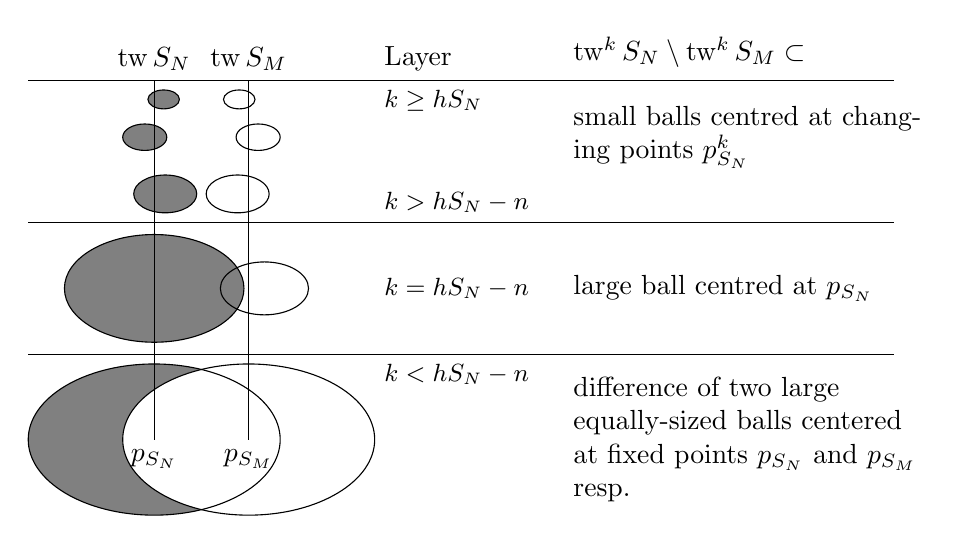
\begin{tikzpicture}[scale=.2,yscale=.6,
					information text/.style={%fill=gray!10,
					inner sep=1ex}]
\def\horizontale{++(55,0)}
\def\yshift{16}
\def\erste{.5*\yshift+1}
\def\yshifteins{10}
\def\yshiftzwei{6}
\def\yshiftdrei{4}
\def\zweite{.5*\yshifteins+2}
\def\gesamt{\yshift+\yshifteins+\yshiftzwei+\yshiftdrei}
\def\senkrechte{\draw (0,0) -- (0,\gesamt+2) node[above]}
\def\textbreite{4.5cm}
%%linker Turm
%%nullte Ebene
\fill[gray] (0,0) circle [radius=8];
%%horizontale
\draw (-8,\erste) -- \horizontale
;
%%erste Ebene
\begin{scope}[yshift=\yshift cm]
\filldraw[fill=gray] (0,0) circle [radius=5.7];
\draw (-8,\zweite) -- \horizontale;
\filldraw[fill=gray] 	++(.7,\yshifteins) circle [radius=2]
					++(-1.3,\yshiftzwei) circle [radius=1.4]
					++(1.2,\yshiftdrei) circle [radius=1];
\end{scope}
\draw (-8,\gesamt+2) -- \horizontale
;
%%rechter Turm
\begin{scope}[xshift=6cm]
%%unterste Ebene
\filldraw[fill=white] (0,0) circle [radius=8];
%%Beschriftung
\draw (8,\erste) node[below right]{\small $k<hS_N-n$};	
\draw		(20,0)node[right, text width=\textbreite]{difference of two large equally-sized balls centered at fixed points $p_{S_N}$ and $p_{S_M}$ resp.};
\begin{scope}[yshift=\yshift cm]
\draw 	(8,0) node[right]{\small $k=hS_N-n$} 
		(8,\zweite)	node[above right]{\small $k>hS_N-n$};
\draw (1,0) circle [radius=2.8]
	 ++(-1.7,\yshifteins) circle [radius=2]
	 ++(1.3,\yshiftzwei) circle [radius=1.4]
	 ++(-1.2,\yshiftdrei) circle [radius=1];
%%Beschriftung
\draw (20,0) node[right
]{large ball centred at $p_{S_N}$}
	 ++(0,\yshifteins+\yshiftzwei) node[right, text width=\textbreite]{small balls centred at changing points $p^k_{S_N}$}
%%Tabellenkopf
	 ++(0,\yshiftdrei+5) node[right]{$\tu^k S_N\setminus \tu^k S_M\subset$};
\end{scope}
\draw (8,\gesamt+2) node[below right]{\small $k\geq hS_N$}
					node[above right]{Layer};
\draw (0,0) node[below] {$p_{S_M}$};
\senkrechte{$\tu{S_M}$};
\end{scope}
%%linker Turm, unterste Ebene, Kreis nachzeichnen
\draw (0,0) node[below] {$p_{S_N}$};
\senkrechte{$\tu{S_N}$};
\draw (0,0) circle [radius=8];
\end{tikzpicture}

\end{document}